%% !TEX root = manual.tex

\section{Launching, Allocation, and Indexing}
\label{sec:tutorial:launchetc}

\subsection{Launch Commands}
\label{subsec:tutorial:launch}
Just as jobs must be launched on a shared supercomputer using Slurm or aprun, 
SST/macro requires the user to specify a launch command for the application.
Currently, we encourage the user to use aprun from Cray, for which documentation can easily be found online.
In the parameter file you specify, e.g.

\begin{ViFile}
app1.name = user_mpiapp_cxx
app1.launch_cmd = aprun -n 8 -N 2
\end{ViFile}
which launches an external user C++ application with eight ranks and two ranks per node.
The aprun command has many command line options (see online documentation), some of which may be supported in future versions of SST/macro.  In particular, we are in the process of adding support for thread affinity, OpenMP thread allocation, and NUMA containment flags.  Most flags, if included, will simply be ignored.

\subsection{Allocation Schemes}
\label{subsec:tutorial:allocation}
In order for a job to launch, it must first allocate nodes to run on. Here we choose a simple 2D torus

\begin{ViFile}
topology.name = torus
topology.geometry = 3 3
topology.concentration = 1
\end{ViFile}
which has 9 nodes arranged in a 3x3 mesh.  
For the launch command \inlinefile{aprun -n 8 -N 2}, we must allocate 4 compute nodes from the pool of 9.
Our first option is to specify the first available allocation scheme (Figure \ref{fig:allocation:first_available})

\begin{ViFile}
app1.launch_allocation = first_available
\end{ViFile}
\begin{figure}[h]
\centering
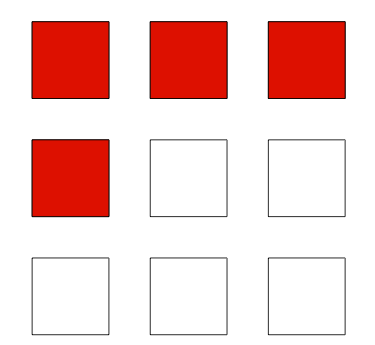
\includegraphics[width=0.35\textwidth]{figures/tikz/allocation/firstavailable.png}
\caption{First available Allocation of 4 Compute Codes on a 3x3 2D Torus}
\label{fig:allocation:first_available}
\end{figure}
In first available, the allocator simply loops through the list of available nodes as they are numbered by the topology object.
In the case of a 2D torus, the topology numbers by looping through columns in a row.
In general, first available will give a contiguous allocation, but it won't necessarily be ideally structured.

To give more structure to the allocation, a Cartesian allocator can be used (Figure \ref{fig:allocation:cartesian}).

\begin{ViFile}
app1.launch_allocation = cartesian
app1.cart_launch_sizes = 2 2
app1.cart_launch_offsets = 0 0
\end{ViFile}
\begin{figure}[h]
\centering
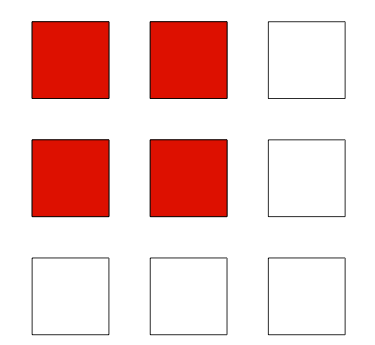
\includegraphics[width=0.35\textwidth]{figures/tikz/allocation/cartesian.png}
\caption{Cartesian Allocation of 4 Compute Codes on a 3x3 2D Torus}
\label{fig:allocation:cartesian}
\end{figure}
Rather than just looping through the list of available nodes, we explicitly allocate a 2x2 block from the torus.
If testing how ``topology agnostic'' your application is, you can also choose a random allocation.

\begin{ViFile}
app1.launch_allocation = random
\end{ViFile}
\begin{figure}[h]
\centering
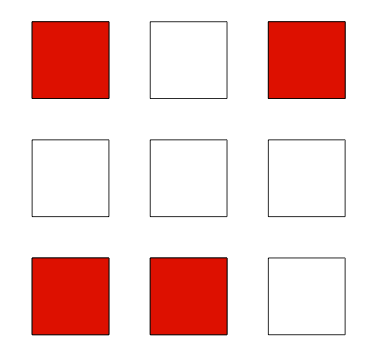
\includegraphics[width=0.35\textwidth]{figures/tikz/allocation/random.png}
\caption{Random Allocation of 4 Compute Codes on a 3x3 2D Torus}
\label{fig:allocation:random}
\end{figure}

In many use cases, the number of allocated nodes equals the total number of nodes in the machine.
In this case, all allocation strategies allocate the same \emph{set} of nodes, i.e. the whole machine.
However, results may still differ slightly since the allocation strategies still assign an initial numbering of the node,
which means a random allocation will give different results from Cartesian and first available.


\subsubsection{Indexing Schemes}
\label{subsec:tutorial:indexing}
Once nodes are allocated, the MPI ranks (or equivalent) must be assigned to physical nodes, i.e. indexed.
The simplest strategies are block and round-robin.  If only running one MPI rank per node, the two strategies are equivalent,
indexing MPI ranks in the order received from the allocation list.
If running multiple MPI ranks per node, block indexing tries to keep consecutive MPI ranks on the same node (Figure \ref{fig:indexing:block}).

\begin{ViFile}
app1.launch_indexing = block
\end{ViFile}
\begin{figure}[h]
\centering
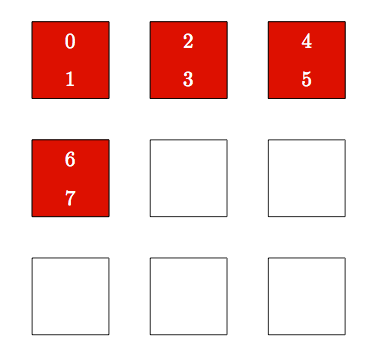
\includegraphics[width=0.4\textwidth]{figures/tikz/indexing/block.png}
\caption{Block Indexing of 8 MPI Ranks on 4 Compute Nodes}
\label{fig:indexing:block}
\end{figure}
In contrast, round-robin spreads out MPI ranks by assigning consecutive MPI ranks on different nodes (Figure \ref{fig:indexing:round_robin}).

\begin{ViFile}
app1.launch_indexing = round_robin
\end{ViFile}
\begin{figure}[h]
\centering
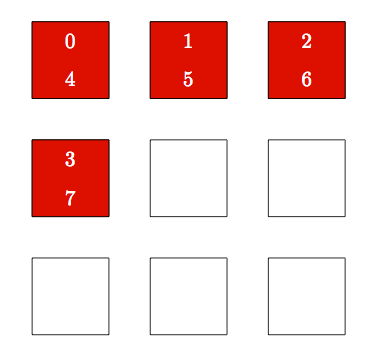
\includegraphics[width=0.4\textwidth]{figures/tikz/indexing/roundrobin.png}
\caption{Round-Robin Indexing of 8 MPI Ranks on 4 Compute Nodes}
\label{fig:indexing:round_robin}
\end{figure}
Finally, one may also choose

\begin{ViFile}
app1.launch_indexing = random
\end{ViFile}
Random allocation with random indexing is somewhat redundant.  
Random allocation with block indexing is \emph{not} similar to Cartesian allocation with random indexing.
Random indexing on a Cartesian allocation still gives a contiguous block of nodes,
even if consecutive MPI ranks are scattered around.
A random allocation (unless allocating the whole machine) will not give a contiguous set of nodes.
